%%% LaTeX Template
%%% This template is made for project reports
%%%	You may adjust it to your own needs/purposes
%%%
%%% Copyright: http://www.howtotex.com/
%%% Date: March 2011

%%% Preamble
\documentclass[10pt]{report}	% Article class of KOMA-script with 11pt font and a4 format

\usepackage[T1]{fontenc}
\usepackage{color}
\usepackage{framed}
\usepackage{textcomp}
\usepackage{listings}
\usepackage{hyperref}
\usepackage[page]{appendix}
\usepackage{graphicx}
\usepackage{verbatim}
\usepackage{amsmath}
\usepackage{xspace}
\usepackage[tt]{titlepic}

\usepackage{sstmacro}

\usepackage[textwidth=7.5in]{geometry}

\definecolor{shadecolor}{rgb}{1,0.8,0.3}
\definecolor{dkgreen}{rgb}{0,0.6,0}
\definecolor{purple}{rgb}{1,0,1}

\newcommand{\todo}[1] {\textcolor{red}{-[#1]-}}


\newcommand{\mytilde}{{\raise.17ex\hbox{$\scriptstyle\sim$}}}

\newcommand{\sstmacro}{{SST/\raise.35ex\hbox{macro}}\xspace}
\newcommand{\eg}{\textit{e.g.}}

\newcommand{\aside}[1]{\begin{framed} #1 \end{framed}}

\newcommand{\inlinefile}[1]{{\lstset{basicstyle=\ttfamily,keywordstyle={}}\lstinline$#1$}}
\newcommand{\inlinecode}[1]{{\lstset{basicstyle=\ttfamily,keywordstyle={},showstringspaces=false}\lstinline$#1$}}
\newcommand{\inlineshell}[1]{{\lstset{basicstyle=\ttfamily,keywordstyle={},showstringspaces=false}\lstinline$#1$}}

\newcommand{\startcpp}{\begin{CppCode}}
\newcommand{\stopcpp}{\end{CppCode}}
\newcommand{\startshell}{\begin{ShellCmd}}
\newcommand{\stopshell}{\end{ShellCmd}}
\newcommand{\startvi}{\begin{ViFile}}
\newcommand{\stopvi}{\end{ViFile}}

\newcommand{\tableConfig}{| p{5cm} | p{2cm} | p{3cm} | p{8cm} |}
\newcommand{\openTable}{\begin{tabular}{\tableConfig}}
\newcommand{\paramType}[1]{\newline (#1)}
\hyphenpenalty=10000
\pagestyle{empty}


\title{SST/macro 8.1: User's Manual}
\titlepic{\includegraphics[width=0.3\textwidth]{figures/sstlogo.png}}
\author{Sandia National Labs \\ Livermore, CA}


\setlength{\parindent}{0cm} % Default is 15pt.
\setlength{\parskip}{2mm plus1mm minus1mm}

\begin{document}
\maketitle 


\tableofcontents
%% !TEX root = manual.tex

\chapter{Introduction}
\label{sec:intro}

\section{Overview}
\label{sec:intro:overview}

The \sstmacro software package provides a simulator for large-scale parallel computer architectures. 
It permits the coarse-grained study of distributed-memory applications. 
The simulator is driven from either a trace file or skeleton application. 
The simulator architecture is modular, allowing it to easily be extended with additional network models, 
trace file formats, software services, and processor models.

Simulation can be broadly categorized as either off-line or on-line.
Off-line simulators typically first run a full parallel application on a real machine,
recording certain communication and computation events to a simulation trace.
This event trace can then be replayed post-mortem in the simulator.
Most common are MPI traces which record all MPI events, and
\sstmacro provides the DUMPI utility (\ref{sec:tutorial:dumpi}) for collecting and replaying MPI traces. 
Trace extrapolation can extend the usefulness of off-line simulation by estimating large or untraceable system scales without   
having to collect a trace, but it is limited.

We turn to on-line simulation when the hardware or applications parameters need to change.
On-line simulators instead run real application code, allowing native C/C++/Fortran to be compiled directly into the simulator.
\sstmacro intercepts certain function calls, estimating how much time passes rather than actually executing the function.
In MPI programs, for example, calls to MPI\_Send are linked to the simulator instead of passing to the real MPI library.
If desired, \sstmacro can actually be a full MPI \emph{emulator}, delivering messages between ranks and replicating the behavior of a full MPI implementation.

Although \sstmacro supports both on-line and off-line modes, on-line simulation is encouraged because
event traces are much less flexible, containing a fixed sequence of events.
Application inputs and number of nodes cannot be changed. 
Without a flexible control flow, it also cannot simulate dynamic behavior like load balancing or faults.
On-line simulation can explore a much broader problem space since they evolve directly in the simulator.

For large, system-level experiments with thousands of network endpoints, high-accuracy cycle-accurate simulation is not possible,
or at least not convenient.
Simulation requires coarse-grained approximations to be practical.
\sstmacro is therefore designed for specific cost/accuracy tradeoffs.
It should still capture complex cause/effect behavior in applications and hardware, but be efficient enough to simulate at the system-level. 
For speeding up simulator execution, we encourage \textit{skeletonization}, discussed further in Chapter \ref{chap:appsAndSkeletonization}. 
A high-quality skeleton is an application model that reproduces certain characteristics with only limited computation.  
We also encourage uncertainty quantification (UQ) for validating simulator results.
Skeletonization and UQ are the two main elements in the ``canonical'' \sstmacro workflow (Figure \ref{fig:workflow}).

\begin{figure}[t]
  \centering
    \includegraphics[width=0.99\columnwidth]{figures/workflow.png}
      \caption{SST/macro workflow.}
      \label{fig:workflow}
\end{figure}

Because of its popularity, MPI is one of our main priorities in providing programming model support.  
Some MPI-3 functions and MPI one-sided functions are not implemented.
This will lead to compile errors with an obvious ``not implement'' compiler message.

\section{Preview of Things to Come}
Suppose you have the basic MPI application below that executes a simple send/recv operation.
One could use \inlineshell{mpicc} or \inlineshell{mpic++} to compile and run as an actual MPI program.
This requires spawning all the processes and running them in parallel.
Suppose, however, you wanted to simulate an entire MPI job launch within a single process.
This might prove very useful for debugging since you could just run GDB or Valgrind on a single process.
It might take a while, but for small runs (16 ranks or so) you could debug right on your laptop the same you do for a serial program.

\begin{CppCode}
int size = atoi(argv[1]);
if (rank == 0){
 int partner = 1;
  MPI_Send(buffer, size, MPI_INT, partner, tag, MPI_COMM_WORLD);
} else {
  int partner = 0;
  MPI_Recv(buffer, size, MPI_INT, partner, tag, MPI_COMM_WORLD, MPI_STATUS_IGNORE);
}
MPI_Barrier(MPI_COMM_WORLD);

if (rank == 0){
  printf("Rank 0 finished at t=%8.4f ms\n", MPI_Wtime()*1e3);
}
\end{CppCode}

This is exactly the functionality that SST/macro provides.
Instead of using \inlineshell{mpic++}, you compile the code with {sst++}.
This modifies your code and intercepts MPI calls, running them through the simulator instead of an actual MPI implementation.
Your code will execute and run exactly the same, and your application won't even know the difference.
You now need a parameter file with information like:

\begin{ViFile}
node {
 app1 {
  name = send_recv
  launch_cmd = aprun -n 2
  argv = 20
 }
}
\end{ViFile}
Rather than launching your code using \inlineshell{mpirun} or similar, you put all your command line parameters into a \inlineshell{parameters.ini} file and run:

\begin{ShellCmd}
shell> sstmac -f parameters.ini
\end{ShellCmd}
The simulator then executes your application exactly as if you had been a real system and run:

\begin{ShellCmd}
shell> aprun -n 2 ./send_recv 20
\end{ShellCmd}
Things get more complicated when you bring skeletonization into play.
The use case above is \emph{emulation}, exactly reproducing MPI functionality.
In \emph{skeletonization} or \emph{simulation}, SST/macro will mimic as closely as possible the original application,
but avoids as much computation and as much memory allocation as possible.
This allows packing in as many simulated (virtual) MPI ranks as possible into your single \inlineshell{sstmac} process.

\section{What To Expect In The User's Manual}
This user's manual is mainly designed for those who wish to perform experiments with \emph{new} applications using \emph{existing} hardware models.
This has been the dominant use case and we therefore classify those doing application experiments as ``users'' and those making new hardware models ``developers.''
Getting applications to run in SST/macro should be very straightforward and requires no knowledge of simulator internal code.
Making new hardware models is much more in depth and requires learning some basics of core simulator code.
Those interested in making new hardware models should consult the developer's manual in the top-level source directory.

%% !TEX root = manual.tex

\chapter{Building and Running SST/macro}
\label{chapter:building}

\section{Build and Installation of \sstmacro}
\label{sec:buildinstall}


\subsection{Downloading}
\label{subsec:build:downloading}

\sstmacro is available at \url{https://github.com/sstsimulator/sst-macro}.
You can download the git repository directly:

\begin{ShellCmd}
shell> git clone https://github.com/sstsimulator/sst-macro.git 
\end{ShellCmd}
or for ssh

\begin{ShellCmd}
shell> git clone ssh://git@github.com/sstsimulator/sst-macro.git 
\end{ShellCmd}
or you can download a release tarball from \url{https://github.com/sstsimulator/sst-macro/releases}.

\subsection{Dependencies}
\label{subsec:build:dependencies}
The most critical change is that C++11 is now a strict prerequisite. 
Workarounds had previously existed for older compilers. 
These are no longer supported.
The following are dependencies for \sstmacro.

\begin{itemize}
\item (optional) Git is needed in order to clone the source code repository, but you can also download a tar (Section \ref{subsec:build:downloading}).
\item Autoconf: 2.68 or later 
\item Automake: 1.11.1 or later 
\item Libtool: 2.4 or later 
\item A C/C++ compiler is required with C++11 support.  gcc >=4.8.5 and clang >= 3.7 are known to work.
\item (optional) OTF2: 2.0 or later for OTF2 trace replay.
\item (optional) VTK 8.1 or later for creating Exodus files for traffic visualization
\item (optional) Paraview 5.0 or greater for visualizing Exodus files
\item (optional) Doxygen and Graphviz are needed to build the source code documentation.
\item (optional) KCacheGrind or QCacheGrind to display call graphs
\item (optional) Clang development libraries to enable SST source-to-source compiler
\end{itemize}

\subsection{Configuration and Building}
\label{subsec:build:configure}

SST/macro is an SST element library, proving a set of simulation components that run on the main SST core.  
The SST core provides the parallel discrete event simulation manager that manages time synchronization and sending events in serial, MPI parallel, multi-threaded, or MPI + threaded mode.  
The core does not provide any simulation components like node models, interconnect models, MPI trace readers, etc.  
The actual simulation models are contained in the element library.  

The SST core is a standalone executable that dynamically loads shared object files containing the element libraries.  
For many element libraries, a Python input file is created that builds and connects the various simulation components.  
For maximum flexibility, this will become the preferred mode.  
However, SST/macro has historically had a text-file input \inlineshell{parameters.ini} that configures the simulation.  
To preserve that mode for existing users, a wrapper Python script is provided that processes SST/macro input files.  
SST/macro can also be compiled in standalone mode that uses its own simulation core.

The workflow for installing and running on the main SST core is:
\begin{itemize}
\item	Build and install SST core
\item Build and install the SST/macro element library \inlineshell{libmacro.so} 
\item Make sure paths are properly configured for \inlineshell{libmacro.so} to be visible to the SST core (\inlineshell{SST_LIB_PATH})
\item Run the \inlineshell{pysstmac} wrapper Python script that runs SST/macro-specific parameters OR
\item Write a custom Python script 
\end{itemize}

The workflow for installing and running on the standalone SST/macro core:
\begin{itemize}
\item Build and install SST/macro standalone to generate \inlineshell{sstmac} executable
\item Run \inlineshell{sstmac} with \inlineshell{*.ini} parameter files
\end{itemize}

\subsubsection{Build SST core}\label{subsec:buildSSTCore}
The recommended mode for maximum flexibility is to run using the SST core downloadable from \url{http://sst-simulator.org/SSTPages/SSTMainDownloads}.
Building and installing sets up the discrete event simulation core required for all SST elements.

\subsubsection{Build SST/macro element library}\label{subsec:buildElementLib}
If using the repo (not a release tarball), go to the top-level source directory and run:
\begin{ShellCmd}
top-level-src> ./bootstrap.sh
\end{ShellCmd}
This sets up the configure script. For builds, we recommend building outside the source tree:

\begin{ShellCmd}
sst-macro> mkdir build
sst-macro> cd build
sst-macro/build> ../configure --prefix=$PATH_TO_INSTALL --with-sst-core=$PATH_TO_SST_CORE CC=$MPICC CXX=$MPICXX
\end{ShellCmd}
\inlinecode{PATH_TO_SST_CORE} should be the prefix install directory used when installing the core.  
The MPI compilers should be the same compilers used for building SST core.

SST/macro can still be built in standalone mode for a select set of features that have not been fully migrated to the SST core.  
The installation and running are the same for both modes - simply remove the \inlineshell{--with--sst-core} parameter.  
A complete list of options for building can be seen by running \inlineshell{../configure --help}.   Some common options for both standalone and main SST core include:

\begin{itemize}
\item --(dis|en)able-graphviz : Enables the collection of simulated call graphs, which can be viewed with graphviz.
Disabled by default.
\item --(dis|en)able-custom-new : Memory is allocated in larger chunks in the simulator, which can speed up large simulations.
\item --(dis|en)able-otf2[=location]: Enable OTF2 trace replay, requires a path to OTF2 installation.
\item --with-clang[=location]: Enable Clang source-to-source tools by pointing to Clang development libraries
\end{itemize}

Once configuration has completed, printing a summary of the things it found, simply type \inlineshell{make}.  

\subsection{Post-Build}
\label{subsec:postbuild}

If the build did not succeed open an issue on the github page at \url{https://github.com/sstsimulator/sst-macro/issues} or contact \sstmacro support for help (sst-macro-help@sandia.gov).

If the build was successful, it is recommended to run the range of tests to make sure nothing went wrong.  
To do this, and also install \sstmacro  to the install path specified during installation, run the following commands:

\begin{ShellCmd}
sst-macro/build> make check
sst-macro/build> make install
sst-macro/build> make installcheck
\end{ShellCmd}
Make check runs all the tests we use for development, which checks all functionality of the simulator.  
Make installcheck compiles some of the skeletons that come with \sstmacro, linking against the installation.  

\aside{
Important:  Applications and other code linking to \sstmacro use Makefiles that use the sst++/sstcc compiler wrappers
that are installed there for convenience to figure out where headers and libraries are.  When making your skeletons and components, make sure your path is properly configured.
}

\subsection{GNU pth for user-space threading: DEPRECATED}\label{subsubsec:pth}
By default, Linux usually ships with \inlineshell{ucontext} which enables user-space threading.
Mac OS X previously required an extra library be installed (GNU pth).
These are no longer required and are deprecated in favor of fcontext,
which is now integrated with the SST/macro distribution (see below).

For those still wishing to use pth, GNU pth is easy to download and install from source.
Even easier is MacPorts. 

\begin{ShellCmd}
shell> sudo port install pth
\end{ShellCmd}

MacPorts installed all libraries to \inlineshell{/opt/local}. 
When configuring, simply add \inlineshell{--with-pth=\$PATH_TO_PTH} as an argument.
For MacPorts installation, this means configuring SST/macro with:

\begin{ShellCmd}
../configure --with-pth=/opt/local
\end{ShellCmd}

\subsection{fcontext}\label{subsubsec:fcontext}
The fcontext library for user-space threading is now integrated directly with the SST/macro distribution.
This provides much greater performance than GNU pth or standard Linux ucontext.
Users may see as much as a 20\% improvement in simulator performance.
fcontext should be activated by default. To force activation fcontext, you can either set the environment variable:

\begin{ShellCmd}
SSTMAC_THREADING=fcontext
\end{ShellCmd}
or in the parameter file specify (more details in Section \ref{sec:parameters}):

\begin{ViFile}
node {
 os {
  context = fcontext
 }
}
\end{ViFile}

\subsection{Known Issues}
\label{subsec:build:issues}


\begin{itemize}
\item Any build or runtime problems should be reported to sst-macro-help@sandia.gov.  We try to respond as quickly as possible.
\item make -j: When doing a parallel compile dependency problems can occur.  
There are a lot of inter-related libraries and files.  
Sometimes the Makefile dependency tracker gets ahead of itself and you will get errors about missing libraries and header files.
If this occurs, restart the compilation.  If the error vanishes, it was a parallel dependency problem.
If the error persists, then it's a real bug.
\item GNU pth: For Mac, make sure to follow directions in \ref{subsubsec:pth} to ensure pth is correctly installed.
\item Ubuntu: The Ubuntu linker performs too much optimization on dynamically linked executables.
Some call it a feature.  I call it a bug.
In the process it throws away symbols it actually needs later. The build system should automatically fix Ubuntu flags.
If still having issues, make sure that '-Wl,--no-as-needed' is given in LDFLAGS.

The problem occurs when the executable depends on libA which depends on libB.
The executable has no direct dependence on any symbols in libB.
Even if you add \inlineshell{-lB} to the \inlineshell{LDFLAGS} or \inlineshell{LDADD} variables,
the linker ignores them and throws the library out.
It takes a dirty hack to force the linkage.
If there are issues, contact the developers at sst-macro-help@sandia.gov and report the problem. 
\end{itemize}

\section{Building DUMPI}
\label{sec:building:dumpi}

By default, DUMPI is configured and built along with SST/macro with support for reading and parsing DUMPI traces, known as libundumpi.  
DUMPI binaries and libraries are also installed along with everything for \sstmacro during make install.   
DUMPI can be used as its own library within the \sstmacro source tree by changing to \inlineshell{sst-macro/sst-dumpi}, 
where you can change its configuration options.  

DUMPI can also be used as stand-alone tool (\eg~for simplicity if you're only tracing). 
To get DUMPI by itself, either copy the \inlineshell{sstmacro/dumpi} directory somewhere else or visit \url{https://github.com/sstsimulator/sst-dumpi} and follow similar instructions for obtaining \sstmacro.

To see a list of configuration options for DUMPI, run \inlineshell{./configure --help}.  
If you're trying to configure DUMPI for trace collection, use \inlineshell{--enable-libdumpi}.
Your build process might look like this (if you're building in a separate directory from the dumpi source tree) :

\begin{ShellCmd}
sst-dumpi/build> ../configure --prefix=/path-to-install --enable-libdumpi
sst-dumpi/build> make
sst-dumpi/build> sudo make install
\end{ShellCmd}

\subsection{Known Issues}
\label{subsubsec:building:dumpi:issues}

\begin{itemize}
\item When compiling on platforms with compiler/linker wrappers, e.g. ftn (Fortran) and CC (C++) compilers 
at NERSC, the libtool configuration can get corrupted.  The linker flags automatically added by the 
wrapper produce bad values for the predeps/postdeps variable in the libtool script in the top 
level source folder.  When this occurs, the (unfortunately) easiest way to fix this is to manually modify
the libtool script.  Search for predeps/postdeps and set the values to empty.
This will clear all the erroneous linker flags.  The compilation/linkage should still work since 
all necessary flags are set by the wrappers. 
\end{itemize}


\section{Building Clang source-to-source support}
\label{sec:buildingClang}

To enable Clang source-to-source support it is not sufficient to have a Clang compiler.  You have to install a special libTooling library for Clang.

\subsection{Building Clang libTooling}
\label{subsec:buildingClanglibTooling}

\subsubsection{The Easy Way: Mac OS X}
\label{subsubsec:libToolingOSX}
Using MacPorts on OS X, it is trivial to obtain a Clang installation that includes libTooling:

\begin{ViFile}
port install clang-devel
\end{ViFile}

MacPorts will place the Clang compilers in \inlineshell{/opt/local/bin}.  Enable the devel version of Clang with:

\begin{ViFile}
port select --set clang mp-clang-devel
\end{ViFile}

The Clang libraries will be placed into \inlineshell{/opt/local/libexec/llvm-devel/lib}, so the appropriate option to the sst-macro configure script is \inlineshell{--with-clang=/opt/local/libexec/llvm-devel}.

\subsubsection{The Hard Way}
\label{subsubsec:libTooling}
For operating systems other than OS X, building Clang support has a few steps (and takes quite a while to build), but is straightforward.
Instead of having an all-in-one tarball, you will have to download several different components. You can install more if you want build libc++, but these are not required.
Obtain the following from \url{http://releases.llvm.org/download.html}.

\begin{itemize}
\item LLVM source code
\item Clang source code
\item libc++ source code
\item libc++abi source code
\item compiler-rt source code
\item (optional, not recommended) OpenMP source code
\end{itemize}

Setting up the folders can be done automatically using the \inlineshell{setup-clang} script in \inlineshell{bin/tools} folder in sst-macro. Put all of downloaded tarballs in a folder, e.g. \inlineshell{clang-llvm}. Then run \inlineshell{setup-clang} in the directory. 
It will automatically place files where LLVM needs them.
LLVM is the ``driver'' for the entire build. Everything else is a subcomponent. 
The setup script places each tarball in the following subfolders of the main LLVM folder

\begin{itemize}
\item tools/clang
\item projects/compiler-rt
\item projects/libcxx
\item projects/libcxxabi
\item projects/openmp
\end{itemize}

Using CMake (assuming you are in a build subdirectory of the LLVM tree), you would run the script below to configure.
You no longer need to use Clang to build Clang. 
For the most stable results, though, you should a pre-existing Clang compiler to build the Clang development libraries.

\begin{ViFile}
cmake ../llvm \
  -DCMAKE_CXX_COMPILER=clang++ \
  -DCMAKE_C_COMPILER=clang \
  -DCMAKE_CXX_FLAGS="-O3" \
  -DCMAKE_C_FLAGS="-O3" \
  -DCMAKE_INSTALL_PREFIX=$install
\end{ViFile}

To build a complete LLVM/Clang run:

\begin{ViFile}
cmake ../llvm \
  -DCMAKE_CXX_COMPILER=clang++ \
  -DCMAKE_C_COMPILER=clang \
  -DCMAKE_CXX_FLAGS="-O3" \
  -DCMAKE_C_FLAGS="-O3" \
  -DLLVM_ENABLE_LIBCXX=ON \
  -DLLVM_TOOL_COMPILER_RT_BUILD=ON \
  -DLLVM_TOOL_LIBCXXABI_BUILD=ON \
  -DLLVM_TOOL_LIBCXX_BUILD=ON \
  -DCMAKE_INSTALL_PREFIX=$install
\end{ViFile}

On some systems, linking Clang might blow out your memory. If that is the case, you have to set \inlineshell{LD=ld.gold} for the linker.
Run \inlineshell{make install}. The libTooling library will now be available at the \inlineshell{\$install} location.

Any compiler used for SST (g++, icpc, clang++) can generally be mixed with most versions of the libtooling source-to-source library.
NOTE: The same compiler used to build SST must have been used to build the libtooling library.
However, the table below contains versions that are recommended or approved and which combinations are untested (but may work).

\begin{tabular}{l l}
\hline
Compiler to build SST & Libtooling version \\
\hline
\hline
Clang 4,5,6 & 4,5,6 \\
Clang 7,8 & 7,8 \\
GCC 4.8-6 & 4-7 \\
GCC 7- & ? \\
 ? & 8 \\
\hline
\end{tabular}

\subsection{Building SST/macro with Clang}
Now that clang is installed, you only need to add the configure flag \inlineshell{--with-clang} pointing it to the install location from above.
You must use the same Clang compiler to build SST that you used to build libTooling.

\begin{ShellCmd}
../configure CXX=clang++ CC=clang --with-clang=$install
\end{ShellCmd}

Clang source-to-source support will now be built into the \inlineshell{sst++} compiler. 
If Clang development libraries are available in the default system path (as is often the case with LLVM models, e..g \inlineshell{module load llvm}),
then you can just put \inlineshell{--with-clang}.

\section{Building with OTF2 (Beta)}
\label{sec:buildingOtf2}
OTF2 is a general purpose trace format with specialized callbacks for the MPI API. OTF2 traces are generated by programs compiled with Score-P compiler wrappers. SST/macro 8.1 supports OTF2 trace replay and OTF2 trace generation when configured with 

\begin{ViFile}
./configure --enable-otf2=<OTF2-root>	
\end{ViFile}
where the OTF2 root is the installation prefix for a valid OTF2 build. OTF2 can be obtained from the Score-P project at {http://www.vi-hps.org/projects/score-p}.
Detailed build and usage instructions can be found on the website.

%\subsection{Building with VTK (Beta)}
%\label{sec:buildingVTK}

\section{Running an Application}\label{sec:building:running}
\subsection{SST Python Scripts}
\label{subsec:SSTPythonScripts}

Full details on building SST Python scripts can be found at \url{http://sst-simulator.org}.  To preserve the old parameter format in the near-term, SST/macro provides the \inlineshell{pysstmac} script:

\begin{ViFile}
export SST_LIB_PATH=$SST_LIB_PATH:$SSTMAC_PREFIX/lib

options="$@"
$SST_PREFIX/bin/sst $SSTMAC_PREFIX/include/python/default.py --model-options="$options"
\end{ViFile}

The script configures the necessary paths and then launches with a Python script \inlineshell{default.py}.  Interested users can look at the details of the Python file to understand how SST/macro converts parameter files into a Python config graph compatible with SST core.
Assuming the path is configured properly, users can run

\begin{ShellCmd}
shell>pysstmac -f parameters.ini
\end{ShellCmd}
with a properly formatted parameter file. If running in standalone mode, the command would be similar (but different).

\begin{ShellCmd}
shell>sstmac -f parameters.ini
\end{ShellCmd}
since there is no Python setup involved.

\subsection{Building Skeleton Applications}
\label{sec:tutorial:runapp}

To demonstrate how an external skeleton application is run in \sstmacro, we'll use a very simple send-recv program located in \inlineshell{skeletons/sendrecv}.
We will take a closer look at the actual code in Section \ref{sec:tutorial:basicmpi}.
After \sstmacro has been installed and your PATH variable set correctly, for standalone core users can run:

\begin{ShellCmd}
sst-macro> cd skeletons/sendrecv
sst-macro/skeletons/sendrecv> make
sst-macro/skeleton/sendrecv> sstmac -f parameters.ini --exe=./runsstmac
\end{ShellCmd}

You should see some output that tells you 1) the estimated total (simulated) runtime of the simulation, and 
2) the wall-time that it took for the simulation to run.  
Both of these numbers should be small since it's a trivial program. 
This is how simulations generally work in \sstmacro: you build skeleton code and link it with the simulator to produce an importable library.  
The importable library contains hooks for loading a skeleton app into the simulator.
NOTE: \inlineshell{runsstmac} appears to be an executable, but is actually built as a shared library. 
If using a regular compiler (e.g. gcc), the Makefile would produce an executable \inlineshell{runsstmac}.
To ensure that building apps for SST require no modification to an existing build system,
SST simple builds a shared library \inlineshell{runsstmac} rather than requiring renaming to the standard convention
\inlineshell{librunsstmac.so}.

\subsection{Makefiles}
\label{subsec:tutorial:makefiles}
We recommend structuring the Makefile for your project like the one seen in \inlineshell{skeletons/sendrecv/Makefile} :

\begin{ViFile}
TARGET := runsstmac
SRC := $(shell ls *.c) 

CXX :=      $(PATH_TO_SST)/bin/sst++
CC :=        $(PATH_TO_SST)/bin/sstcc
CXXFLAGS := ...
CPPFLAGS := ...
LIBDIR :=  ...
PREFIX :=   ...
LDFLAGS :=  -Wl,-rpath,$(PREFIX)/lib
...
\end{ViFile}
The SST compiler wrappers \inlineshell{sst++} and \inlineshell{sstcc} automagically configure and map the code for simulation. 

\subsection{Command-line arguments}
\label{subsec:tutorial:cmdline}

There are few common command-line arguments with \sstmacro, listed below

\begin{itemize}
\item -h/--help: Print some typical help info
\item -f [parameter file]: The parameter file to use for the simulation.  
This can be relative to the current directory, an absolute path, or the name of a pre-set file that is in sstmacro/configurations 
(which installs to /path-to-install/include/configurations, and gets searched along with current directory). 
\item --dumpi: If you are in a folder with all the DUMPI traces, you can invoke the main \inlinecode{sstmac} executable with this option.  This replays the trace in a special debug mode for quickly validating the correctness of a trace.
\item --otf2: If you are in a folder with all the OTF2 traces, you can invoke the main \inlinecode{sstmac} executable with this option.  This replays the trace in a special debug mode for quickly validating the correctness of a trace.
\item -d [debug flags]: A list of debug flags to activate as a comma-separated list (no spaces) - see Section \ref{sec:dbgoutput}
\item -p [parameter]=[value]: Setting a parameter value (overrides what is in the parameter file)
\item -t [value]: Stop the simulation at simulated time [value]
\item -c: If multithreaded, give a comma-separated list (no spaces) of the core affinities to use - see Section \ref{subsec:parallelopt}
\end{itemize}

\section{Parallel Simulations in Standalone Mode}
\label{sec:PDES}

\sstmacro supports running parallel discrete event simulation (PDES) in distributed memory (MPI), threaded shared memory (pthreads) and hybrid (MPI+pthreads) modes.  Running these in standalone mode will be discouraged as parallel simulations should use the unified SST core. However, near-term, hybrid modes and other optimizations are not fully supported in the unified SST core. The standalone core may still be required for certain cases.

\subsection{Distributed Memory Parallel}
\label{subsec:mpiparallel}
Configure will automatically check for MPI.
Your configure should look something like:

\begin{ShellCmd}
sst-macro/build> ../configure CXX=mpicxx CC=mpicc ...
\end{ShellCmd}
With the above options, you can just compile and go.
\sstmacro is run exactly like the serial version, but is spawned like any other MPI parallel program.
Use your favorite MPI launcher to run, e.g. for OpenMPI

\begin{ShellCmd}
mysim> mpirun -n 4 sstmac -f parameters.ini
\end{ShellCmd}
or for MPICH

\begin{ShellCmd}
mysim> mpiexec -n 4 sstmac -f parameters.ini
\end{ShellCmd}

Even if you compile for MPI parallelism, the code can still be run in serial with the same configuration options.
\sstmacro will notice the total number of ranks is 1 and ignore any parallel options.
When launched with multiple MPI ranks, \sstmacro will automatically figure out how many partitions (MPI processes) 
you are using, partition the network topology into contiguous blocks, and start running in parallel.   

\subsection{Shared Memory Parallel}
\label{subsec:parallelopt}
In order to run shared memory parallel, you must configure the simulator with the \inlineshell{--enable-multithread} flag.
Partitioning for threads is currently always done using block partitioning and there is no need to set an input parameter.
Including the integer parameter \inlineshell{sst_nthread} specifies the number of threads to be used (per rank in MPI+pthreads mode) in the simulation.
The following configuration options may provide better threaded performance.
\begin{itemize}
\item\inlineshell{--enable-spinlock} replaces pthread mutexes with spinlocks.  Higher performance and recommended when supported.
\item\inlineshell{--enable-cpu-affinity} causes \sstmacro to pin threads to specific cpu cores.  When enabled, \sstmacro will require the
\inlineshell{cpu_affinity} parameter, which is a comma separated list of cpu affinities for each MPI task on a node.  \sstmacro will sequentially
pin each thread spawned by a task to the next next higher core number.  For example, with two MPI tasks per node and four threads per MPI task,
\inlineshell{cpu_affinity = 0,4} will result in MPI tasks pinned to cores 0 and 4, with pthreads pinned to cores 1-3 and 5-7.
For a threaded only simulation \inlineshell{cpu_affinity = 4} would pin the main process to core 4 and any threads to cores 5 and up.
The affinities can also be specified on the command line using the \inlineshell{-c} option.
Job launchers may in some cases provide duplicate functionality and either method can be used.
\end{itemize}

\subsection{Warnings for Parallel Simulation}
\label{subsec:parallelwarn}
\begin{itemize}
\item If the number of simulated processes specified by e.g. \inlinefile{aprun -n 100} does not match the number of nodes in the topology (i.e. you are not space-filling the whole simulated machine), parallel performance will suffer. \sstmacro partitions nodes, not MPI ranks.
\end{itemize}

\aside{
Parallel simulation speedups are likely to be modest for small runs.
Speeds are best with serious congestion or heavy interconnect traffic.
Weak scaling is usually achievable with 100-500 simulated MPI ranks per logical process.
Even without speedup, parallel simulation can certainly be useful in overcoming memory constraints.
}

\section{Debug Output}
\label{sec:dbgoutput}
\sstmacro defines a set of debug flags that can be specified in the parameter file to control debug output printed by the simulator.
To list the set of all valid flags with documentation, the user can run

\begin{ShellCmd}
bin> ./sstmac --debug-flags
\end{ShellCmd}

which will output something like

\begin{ViFile}
    mpi
        print all the basic operations that occur on each rank - only API calls are
        logged, not any implementation details
    router
        print all operations occurring in the router
     ....
\end{ViFile}


To turn on debug output, add the following to the input file

\begin{ViFile}
debug = mpi 
\end{ViFile}
listing all flags you want separated by spaces.


\input{Tutorials}
%% !TEX root = manual.tex

\chapter{Topologies}
\label{chapter:topologies}


The torus topology is straightforward and easy to understand.
Here we introduce the basics of other topologies within SST that are more complex and require extra documentation to configure properly.
These are generally higher-radix or path-diverse topologies like fat tree, dragonfly, and flattened butterfly.  
As noted in \ref{sec:tutorial:topology}, a more thorough and excellent discussions of these topologies is given in ``High Performance Datacenter Networks'' by Dennis Abts and John Kim.

%\section{Topology Query Utility}
%\label{sec:topologyQuery}
%Understanding topology inputs and geometries can sometimes be challenging.
%\sstmacro provides an executable for testing topology inputs and doing example coordinate computations.
%After making and installing, an executable \inlineshell{sstmac_top_info} will appear in the \inlineshell{bin} folder.
%The invocation of \inlineshell{sstmac_top_info} is exactly the same as the main \inlineshell{sstmac} executable.
%For the example parameter file named \inlineshell{machine.ini}:
%
%\begin{ViFile}
%topology.name = fat_tree
%topology.geometry = 4 3
%\end{ViFile}
%
%we run
%
%\begin{ShellCmd}
%bin> sstmac_top_info -f machine.ini
%\end{ShellCmd}
%which produces the output
%
%\begin{ViFile}
%Number of nodes:         81
%Number of leaf switches: 27
%Number of switches:      94
%\end{ViFile}
%
%detailing the produced geometry.  Here the fat tree has a total of 94 switches, 27 of which are ``leaf'' switches directly connected to compute nodes.
%The output is followed by the prompt
%
%\begin{ShellCmd}
%NextInput: 
%\end{ShellCmd}
%
%One can either enter a single number (switch ID) or set of coordinates.
%If given a switch ID, the coordinates are computed.
%If coordinates are given, the switch ID is computed.
%
%\begin{ShellCmd}
%NextInput: 32
%Switch ID maps to coordinates [ 2 0 1 2 ]
%NextInput: 2 0 1 2
%Coordinates map to switch ID 32
%\end{ShellCmd}
%
%The program is just exited with Ctrl-C.
%The meaning of the above coordinates is detail below for fat tree (Section \ref{sec:tutorial:fattree}).


\input{Torus}
\input{Hypercube}
%% !TEX root = manual.tex

\section{Fat Tree}
\label{sec:tutorial:fattree}

SST provides a very flexible fat-tree topology which allows both full bandwidth and tapered bandwidth configurations using either uniform or non-uniform switches.  
This flexibility requires a farily complicated set of input parameters which are best introduced by examining a couple of example configurations.  Consider the full-bandwidth topology in Figure~\ref{fig:topologies:fullfattree} which uses uniform 8-port switches throughout.

\begin{figure}[h!]
\centering
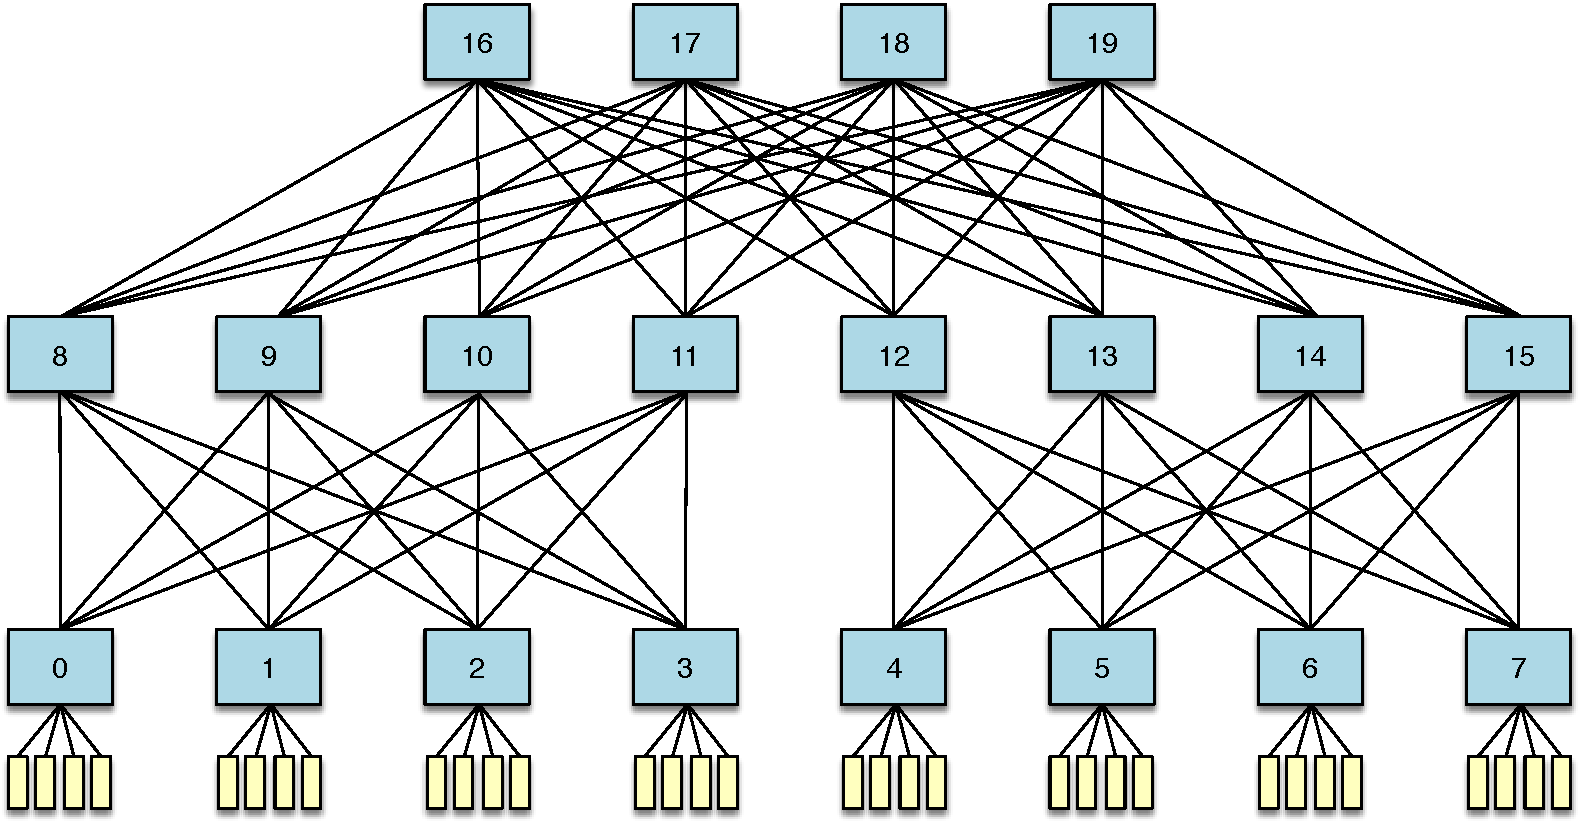
\includegraphics[width=0.7\textwidth]{figures/topologies/fattree4.pdf}
\caption{Full-bandwidth fat-tree topology using uniform 8-port switches.}
\label{fig:topologies:fullfattree}
\end{figure}

The SST fat-tree is strictly a 3-level topology, with the switch levels refered to as leaf (bottom), aggregation (middle), and core (top).
Interconnected leaf and aggregation switches form an aggregation subtree, which forms the basic unit of a fat-tree topology.
The structure of the aggregation subtree is, itself, flexible and places few constraints on the number of subtrees or the way they are connected to the core level.
In Figure~\ref{fig:topologies:fullfattree}, there are 4 leaf switches and 4 aggregation switches per subtree, and each leaf switch has a concentration of four nodes per switch.
Balancing bandwidth, there are 4 ports going up from each leaf switch and 4 ports going down from each aggregation switch.
This subtree can be specified as follows:

\begin{ViFile}
topology.leaf_switches_per_subtree = 4
topology.agg_switches_per_subtree = 4
topology.concentration = 4
topology.up_ports_per_leaf_switch = 4
topology.down_ports_per_agg_switch = 4
\end{ViFile}

In this example we have 2 aggregation subtrees.
There are four ports going up from each aggregation switch.
All of the ports on the core switches go down, so the number of core switches required (4) is only half the number of total aggregation switches (8).
This core configuration can be specified as follows:

\begin{ViFile}
topologies.num_agg_subtrees = 2
topologies.num_core_switches = 4
topologies.up_ports_per_agg_switch = 4
topologies.down_ports_per_core_switch = 8
\end{ViFile}

Putting it all together with the topology name results in:

\begin{ViFile}
topology.name = fat_tree
logy.leaf_switches_per_subtree = 4
topology.agg_switches_per_subtree = 4
topology.concentration = 4
topology.up_ports_per_leaf_switch = 4
topology.down_ports_per_agg_switch = 4
topologies.num_agg_subtrees = 2
topologies.num_core_switches = 4
topologies.up_ports_per_agg_switch = 4
topologies.down_ports_per_core_switch = 8
\end{ViFile}

The next example, though somewhat contrived, better demonstrates the fat-tree input flexibility.
Suppose that one wanted to use the same 8-port switches to construct a 3-level fat-tree that was both cheaper and had more endpoints (nodes), at the cost of interswitch bandwidth.
One possible configuration is shown in Figure~\ref{fig:topologies:taperedfattree}.

\begin{figure}[h!]
\centering
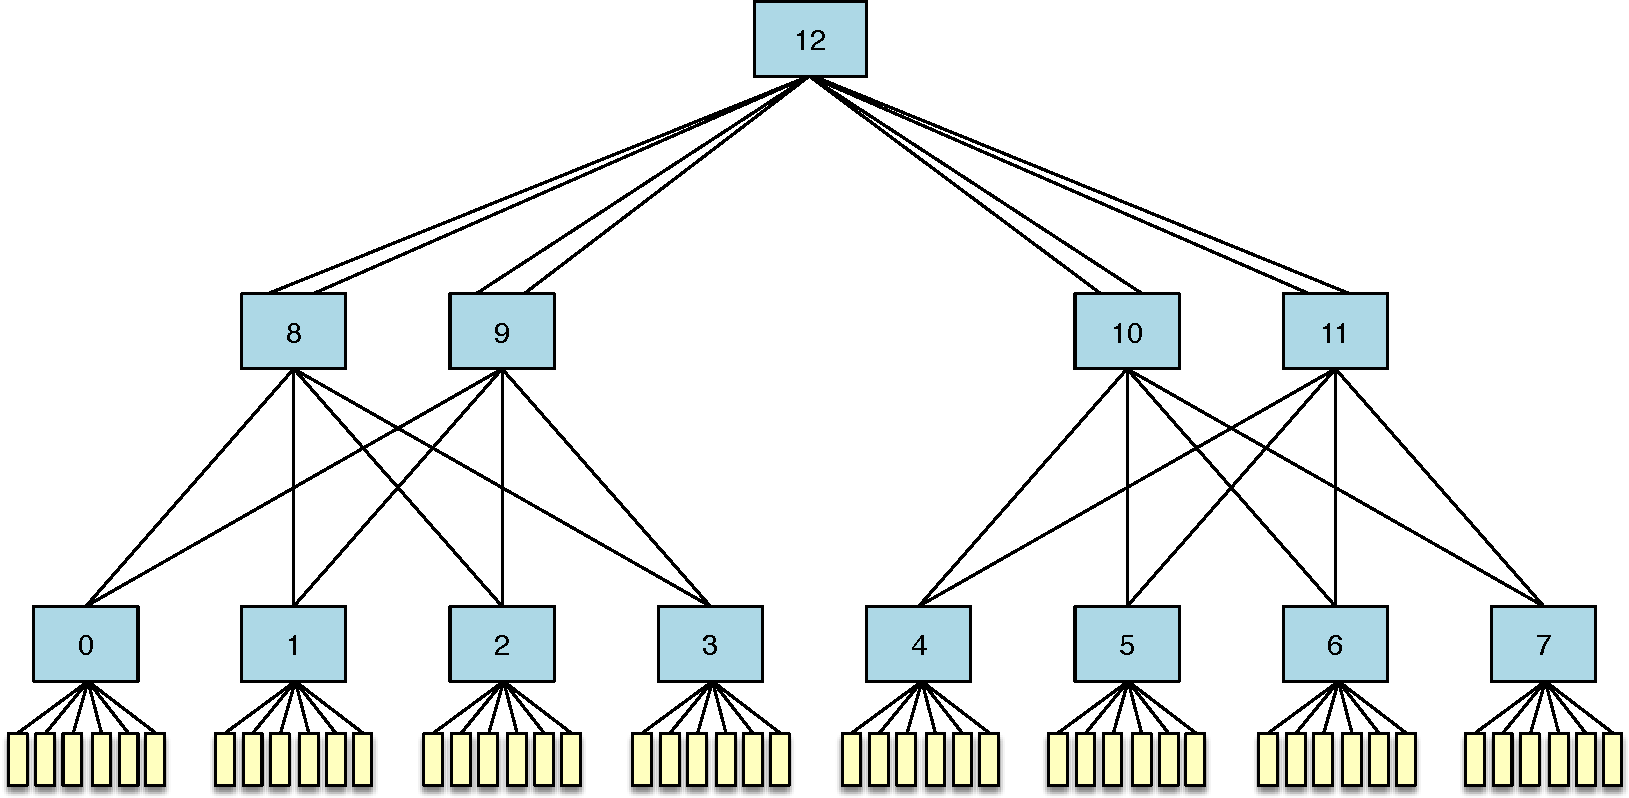
\includegraphics[width=0.7\textwidth]{figures/topologies/fattree4-tapered.pdf}
\caption{A tapered fat-tree topology using uniform 8-port switches.}
\label{fig:topologies:taperedfattree}
\end{figure}

Here the concentration has been increased to 6 nodes per leaf switch, leaving only two up ports per leaf switch.
Thus an aggregation subtree has a total of only 8 leaf up ports, which requires at least two aggregation switches (in order to have any ports left to connect into the core).
Each aggregation switch is then required to have 4 ports heading down.
The subtree can be configured as follows:

\begin{ViFile}
topology.leaf_switches_per_subtree = 4
topology.agg_switches_per_subtree = 2
topology.concentration = 6
topology.up_ports_per_leaf_switch = 2
topology.down_ports_per_agg_switch = 4
\end{ViFile}

There are a total of four aggregation switches.
If the bandwidth is allowed to taper again, a single 8-port core switch can accomodate 2 ports coming up from each aggregation switch.
This core configuration can be specified as follows:

\begin{ViFile}
topologies.num_agg_subtrees = 2
topologies.num_core_switches = 1
topologies.up_ports_per_agg_switch = 2
topologies.down_ports_per_core_switch = 8
\end{ViFile}

This is a heavily tapered tree and also has the downside of using only 6 ports per switch in the aggregation level.
This example was chosen more for its illustrative rather than practical value, though there are certainly applications where it would be perfectly adequate. 
More practical tapering becomes an option when you increase the number of ports per switch, but visualizations become more difficult to grasp.

The following constraints must be met for a valid configuration.
\begin{itemize}
\renewcommand{\labelitemii}{$\circ$}
\item Down ports must equal up ports: leaf up ports (\inlineshell{leaf_switches_per_subtree} $\cdot$ \inlineshell{up_ports_per_leaf_switch}) must equal aggregation down ports (\inlineshell{agg_switches_per_subtree} $\cdot$ \inlineshell{down_ports_per_agg_switch}), and total aggregation up ports (\inlineshell{up_ports_per_agg_switch} $\cdot$ \inlineshell{agg_switches_per_subtree} $\cdot$ \inlineshell{num_agg_subtrees}) must equal total core down ports (\inlineshell{num_core_switches} $\cdot$ \inlineshell{down_ports_per_core_switch}).
\item Need enough down ports -- each switch must have at least one link into each "unit" (subtree or switch, depending on level) below it:  \inlineshell{down_ports_per_core_switch} must be $\geq$ \inlineshell{num_agg_subtrees}, and \inlineshell{down_ports_per_agg_switch} must be $\geq$ \inlineshell{leaf_switches_per_subtree}.
\item Need enough up ports -- each "unit" (subtree or switch) must have at least one link into each switch above it: \inlineshell{up_ports_per_agg_switch} $\cdot$ \inlineshell{agg_switches_per_subtree} must be $\geq$ \inlineshell{num_core_switches}, and \inlineshell{up_ports_per_leaf_switch} must be $\geq$ \inlineshell{agg_switches_per_subtree}.
\item Connections need to be regular:
  \begin{itemize}
  \item \inlineshell{down_ports_per_core_switch} $\bmod$ \inlineshell{num_agg_subtrees} must equal zero
  \item \inlineshell{down_ports_per_agg_switch} $\bmod$ \inlineshell{leaf_switches_per_subtree} must equal zero
  \item \inlineshell{up_ports_per_leaf_switch} $\bmod$ \inlineshell{agg_switches_per_subtree} must equal zero
  \end{itemize}
\end{itemize}

\subsection{Switch Crossbar Bandwidth Scaling}
\label{subsec:fattree:xbarbw}

Allowing non-uniform switches in the topology implies that switch crossbar bandwidth should be non-uniform as well.
By default, SST assumes \inlineshell{switch.xbar.bandwidth} specifies the bandwidth for the switch type with the lowest port count.
The crossbar bandwidth is scaled by the total number of ports for all other switch types. 
Input keywords are provided to override this default behavior.
For the tapered-bandwidth example above, uniform switch bandwidth can be maintained by setting all bandwidth scaling to 1.0:

\begin{ViFile}
topology.leaf_bandwidth_multiplier = 1.0
topology.agg_bandwidth_multiplier = 1.0
topology.core_bandwidth_multiplier = 1.0
\end{ViFile}

\subsection{Routing}
\label{subsec:fattree:routing}

The fat-tree topology should be used in conjunction with \inlineshell{router = fat_tree}, which will maximize the utilization of path diversity.
There is a \inlineshell{fat_tree_minimal} router which will use the lowest numbered valid port for any destination; this will result in poor network performance and is primarily useful for testing and perhaps experiments where network contention is desired.

\input{Cascade}



% !TEX root = manual.tex

\chapter{External Applications and Skeletonization}
\label{chap:appsAndSkeletonization}

\section{Basic Application porting}
\label{sec:skel:basic}
There are three parts to successfully taking a C++ code and turning it into a scalable simulation.
\begin{itemize}
\item Symbol Interception: Rather than linking to MPI, pThreads, or other parallel libraries (or even calling \inlinecode{hostname}), these functions must be redirected to \sstmacro rather than calling the native libraries on the machine running the simulator.
You get all redirected linkage for free by using
the SST compiler wrappers \inlineshell{sst++} and \inlineshell{sstcc} installed in the \inlineshell{bin} folder.
\item Skeletonization: While \sstmacro can run in emulation mode, executing your entire application exactly, this is not scalable.  To simulate at scale (i.e. 1K or more MPI ranks) you must strip down or ``skeletonize'' the application to the minimal amount of computation.  The energy and time cost of expensive compute kernels are then simulated via models rather than explicitly executed. 
\item Process encapsulation: Each virtual process being simulated is not an actual physical process. It is instead modeled as a lightweight user-space thread.  This means each virtual process has its own stack and register variables, but not its own data segment (global variables).
Virtual processes share the same address space and the same global variables.  A Beta version of the auto-skeletonizing clang-based SST compiler is available with the 7.X releases. If the Beta is not stable with your application, manual refactoring may be necessary if you have global variables.
\end{itemize}

Now in Beta, another possible feature is available:
\begin{itemize}
\item Memoization hooks: Rather than building an app for simulation, build an app with special profiling hooks. There is no skeletonization or redirected linkage, but the runtime or performance counters obtained by running should be used to build models for simulation.
\end{itemize}

There are generally 3 modes of using an application common with SST/macro:
\begin{itemize}
\item Simulation: As lightweight as possible without sacrificing accuracy. Intended to be used for performance estimation at large scales.
\item Emulation/Virtualization: Run a parallel or distributed application within a single simulator thread/process - primarily useful for debugging.
\item Memoization: Run a full application within the simulator, collecting performance counters or timers on critical sections
\end{itemize}

\begin{center}
\begin{tabular}{l l l l l}
\hline
 & Simulator hooks & Symbol interception & Skeletonization & Process encapsulation \\
\hline
\hline
Simulation & Yes & Yes & Yes & Yes \\
Virtualization & Yes & Yes & No & Yes \\
Memoization & Yes & No & No & No \\
\hline
\end{tabular}
\end{center}

\subsection{Loading external skeletons with the standalone core}\label{subsec:externalAppStandalone}
You should always write your own skeleton applications in an external folder rather then integrating directly into the \inlineshell{sstmac} executable.
Existing make systems can be used unmodified. Rather than producing an executable, though, SST/macro produces a shared library.
These shared libraries are then imported into the main \inlinecode{sstmac} executable.

If you follow the example in the \inlineshell{skeletons/sendrecv} folder,
the Makefile shows how to generate an importable skeleton.
If you are using \inlineshell{sst++}, it will automatically convert executables into loadable libraries.
If your application is named \inlineshell{runapp}, you would run it with \inlineshell{sstmac}:

\begin{ShellCmd}
./runapp -f parameters.ini --exe=./runapp
\end{ShellCmd}
directing to load the library as a skeleton executable.

\section{Auto-skeletonization with Clang}
\label{sec:autoSkeletonization}

The build of the Clang toolchain is described in Section \ref{sec:buildingClang}. 
This enables a source-to-source translation capability in the \inlineshell{sst++} compiler that can auto-skeletonize computation and fix global variable references.
Some of this can be accomplished automatically (global variables), but most of it (removing computation and memory allocations) must occur through pragmas.
A good example of skeletonization can be found in the lulesh2.0.3 example in the skeletons folder. Most of the available SST pragmas are used there.
Pragmas are preferred since they allow switching easily back and forth between skeleton and full applications.
This allows much easier validation of the simulation. The section here briefly introduces the SST pragma language.
A complete tutorial on all available pragmas is given in Chapter \ref{clangTutorial}.

\subsection{Redirecting Main}
Your application's \inlinecode{main} has to have its symbols changed.
The simulator itself takes over \inlinecode{main}.
\sstmacro therefore has to capture the function pointer in your code and associate it with a string name for the input file.
This is automatically accomplished by defining the macro \inlinecode{sstmac_app_name} either in your code or through a \inlineshell{-D=} build flag to the name of your application (unquoted!). The value of the macro will become the string name used for launching the application via \inlinecode{node.app1.name=X}.
Even without Clang, this works for C++. For C, Clang source-to-source is required.

\subsection{Memory Allocations}
To deactivate memory allocations in C code that uses \inlinecode{malloc}, use:
\begin{CppCode}
#pragma sst malloc
  void* ptr = malloc(...)
\end{CppCode}
prior to any memory allocations that should be deactivated during skeleton runs, but active during real runs.

Similarly, for C++ we have
\begin{CppCode}
#pragma sst new
  int* ptr = new int[...]
\end{CppCode}

\subsection{Computation}
In general, the SST compiler captures all \inlinecode{#pragma omp parallel} statements.
It then analyzes the for-loop or code block and attempts to derive a computational model for it.
The computational models are quite simple (skeleton apps!), 
based simply on the number of flops executed and the number of bytes read (written) from memory.
Consider the example:

\begin{CppCode}
double A[N], B[N];
#pragma omp parallel for
for (int i=0; i < N; ++i){
  A[i] = alpha*A[i] + B[i];
}
\end{CppCode}
The SST compiler deduces $16N$ bytes read, $8N$ bytes written, and $16N$ flops (or $8N$ if fused-multiplies are enabled).
Based on processor speed and memory speed, it then estimates how long the kernel will take without actually executing the loop.
If not wanting to use OpenMP in the code, \inlinecode{#pragma sst compute} can be used instead of \inlinecode{#pragma omp parallel}.

\subsection{Special Pragmas}
Many special cases can arise that break skeletonization.
This is often not a limit of the SST compiler, but rather a fundemental limitation in the static analysis of the code.
This most often arises due to nested loops. Consider the example:

\begin{CppCode}
#pragma omp parallel for
for (int i=0; i < N; ++i){
  int nElems = nElemLookup[i];
  for (int e=0; e < nElems; ++e){
  }
}
\end{CppCode}
Auto-skeletonization will fail. The skeletonization converts the outer loop into a single call to an SST compute model.
However, the inner loop can vary depending on the index.
This data-dependency breaks the static analysis.
To fix this, a hint must be given to SST as to what the ``average'' inner loop size is.
For example, it may loops nodes in a mesh. In this case, it may almost always be 8.

\begin{CppCode}
#pragma omp parallel for
for (int i=0; i < N; ++i){
  int nElems = nElemLookup[i];
  #sst replace nElems 8
  for (int e=0; e < nElems; ++e){
  }
}
\end{CppCode}
This hint allows SST to skeletonize the inner loop and ``guess'' at the data dependency.



\subsection{Skeletonization Issues}
\label{subsec:skeletonIssues}
Skeletonization challenges fall into three main categories:

\begin{itemize}
\item \textit{Data structures} - Memory is a precious commodity when running large simulations, so get rid of every memory allocation you can.
\item \textit{Loops} - Usually the main brunt of CPU time, so get rid of any loops that don't contain MPI calls or calculate variables needed in MPI calls.
\item \textit{Communication buffers} - While you can pass in real buffers with data to \sstmacro MPI calls and they will work like normal, it is relatively expensive. If they're not needed, get rid of them.
\end{itemize}





The main issue that arises during skeletonization is data-dependent communication.  
In many cases, it will seem like you can't remove computation or memory allocation because MPI calls depend somehow on that data.  
The following are some examples of how we deal with those:

\begin{itemize}
\item \textit{Loop convergence} - In some algorithms, the number of times you iterate through the main loop depends on an error converging to near zero, or some other converging mechanism.  This basically means you can't take out anything at all, because the final result of the computation dictates the number of loops.  In this case, we usually set the number of main loop iterations to a fixed number.  
\item \textit{Particle migration} - Some codes have a particle-in-cell structure, where the spatial domain is decomposed among processes, and particles or elements are distributed among them, and forces between particles are calculated.  When a particle moves to another domain/process, how many particles migrate and how far depends on the actual computed forces. However, in the skeleton, we are not actually computing the forces - only estimated how long the force computation took.  If all we need to know is that this migration/communication happens sometimes, then we can just make it happen every so many iterations, or even sample from a probability distribution.  
\item \textit{AMR} - Some applications, like adaptive mesh refinement (AMR), exhibit communication that is entirely dependent on the computation.  In this case, skeletonization again depends on making approximations or probability estimates of where and when box refinement occurs without actually computing everything.
\end{itemize}

For applications with heavy dynamic data dependence, we have the following strategies:
\begin{itemize}
\item \textit{Traces}  - revert to DUMPI traces, where you will be limited by existing machine size.  Trace extrapolation is also an option here.
\item \textit{Synthetic} - It may be possible to replace communication with randomly-generated data and decisions, which emulate how the original application worked. This occurs in the CoMD skeleton.
\item \textit{Hybrid} - It is possible to construct meta-traces that describe the problem from a real run, and read them into \sstmacro to reconstruct the communication that happens.  This occurs in the \inlineshell{boxml} aplications.
\end{itemize}

\section{Process Encapsulation}
\label{sec:processEncapsulation}
As mentioned above, virtual processes are not real, physical processes inside the OS.
They are explicitly managed user-space threads with a private stack, but without a private set of global variables.
When porting an application to SST/macro, global variables used in C programs will not be mapped to separate memory addresses causing incorrect execution or even segmentation faults.
If you have avoided global variables, there is no major issue.  
If you have read-only global variables with the same value on each machine, there is still no issue.
If you have mutable global variables, you should use the \inlineshell{sst++} clang-based compiler wrappers to auto-refactor your code (Section \ref{sec:autoSkeletonization}).
This feature is current labeled Beta, but is stable for numerous tests and will be fully supported for release 7.1.


%% !TEX root = manual.tex

\chapter{Clang Source-to-Source Auto-Skeletonization via Pragmas}
\label{clangTutorial}

There are three main examples of auto-skeletonization with pragmas in the \sstmacro source code in the \inlineshell{skeletons} directory.
These applications are Lulesh, HPCG, and CoMD.
The auto-skeletonizing compiler is designed to do three main things:

\begin{itemize}
\item Redirect global variable accesses to thread-specific values
\item Turn off large memory allocations that would prevent scalable simulation
\item Estimate time of compute-intensive kernels instead of executing them
\end{itemize}

\section{Pragma Overview}

\begin{figure}[h!]
\centering
\includegraphics[width=0.66\textwidth]{figures/compilerWorkflow}
\caption{Source-to-source transformation workflow for SST compiler. For C source files, g++ can be swapped with gcc. The choice of underlying compiler is actually arbitrary and can be clang, gcc, icc, etc.}
\label{fig:compilerWorkflow}
\end{figure}

\subsection{Compiler workflow}
The source-to-source compiler operates on a pre-processed source file.
The source code transformation generates a temporary source file.
This temporary source file is then compiled into the target object file.
Global variables require static registration of C++ variables.
Here another temporary C++ source file (even if the original file is C)
is generated that has all static global variable registrations.
The corresponding object file is merged with the original object file,
creating a complete \sstmacro object file with the transformed code and C++ static registrations.
This workflow is shown in Figure \ref{fig:compilerWorkflow}.

\subsection{Compiler Environment Variables}

\subsubsection{SSTMAC\_SRC2SRC: Default 1}
If set to zero, deactivates the source-to-source transformation. 
The compiler wrapper will then compile the code into the simulator, but will not redirect any global variable accesses or perform any skeletonization.

\subsubsection{SSTMAC\_SKELETONIZE: Default 0}
If set to zero, deactivates skeletonization. 
This does not deactivate global variable redirection.
Thus, with \inlineshell{SSTMAC_SRC2SRC=1} and \inlineshell{SSTMAC_SKELETONIZE=0},
\sstmacro will act as an MPI emulator executing a full code but with global variables refactored to maintain correctness.

\subsubsection{SSTMAC\_MEMOIZE: Default 0}
If set to nonzero, activates memoization hooks. 
This deactivates all global variable refactoring, all symbol interception, and all skeletonization.

\subsubsection{SSTMAC\_HEADERS: No default}
The compiler wrapper will only redirect global variables that it knows should definitely be modified.
All global variables found in source files will be redirected.
\inlinecode{extern} global variables found in header files are more difficult.
Certain system global variables like \inlinecode{stderr} should not be modified and so are left as global variable constants.
By default, global variables in a header file are NOT redirected unless explicitly specified in a header configuration file.
The variable \inlineshell{SSTMAC_HEADERS} should give the full path of a file containing the list of header files.
Header file paths in the file should be one per line and should be the full path, not a relative path.

\subsubsection{SSTMAC\_DELETE\_TEMPS: Default 1}
If non-zero, the compiler cleans up all temporary files. 
If you wish to keep temporary files to view them for debugging, set to zero.
All temporary, intermediate source files will otherwise be deleted at the end of compilation.

\section{Basic Replacement Pragmas}
When skeletonization is active (see \inlineshell{SSTMAC_SKELETONIZE}), these pragmas will cause replacements in the original source code.
Pragmas appy to the next statement in the source code.
For compound statements such as a for-loop with a multi-statement body, the pragma applies to the entire for-loop.
\subsection{pragma sst delete: no arguments}
This deletes the next statement from the source code.
If the statement declares a variable that is used later in the code, this will cause a compile error.
Consider an example from the Lulesh source code.

\begin{CppCode}
#pragma sst delete
    testnorms_data.values[i] = normr/normr0;
\end{CppCode}
In the skeleton, the residual is not actually computed and the \inlinecode{testnorms_data} array is not actually allocated.
Thus this statement should be deleted and not actually executed in the skeleton.

\subsection{pragma sst replace [to\_replace:string] [new\_text:C++ expression]}
This applies a string replace to a variable or function call in the next statement.
Consider an example from Lulesh.

\begin{CppCode}
#pragma sst replace volo 1
   deltatime() = (Real_t(.5)*cbrt(volo(0)))/sqrt(Real_t(2.0)*einit);
\end{CppCode}
The function call \inlinecode{volo(0)} is not valid in the skeleton since volumes are not actually computed.
Here we simply estimate that all cells have unit volume replacing \inlinecode{volo(0)} with \inlinecode{1}.

\subsection{pragma sst init [new\_value:string]}
This pragma can only apply to a binary equals operator assigning a value.
The pragma changes the right-hand side to use the given new value.
For example, in Lulesh:

\begin{CppCode}
#pragma sst init nullptr
  destAddr = &domain.commDataSend[pmsg * maxPlaneComm] ;
\end{CppCode}
The send buffer \inlinecode{domain.commDataSend} is not allocated in the skeleton and thus is not valid to use.
The pragma causes the skeleton to simply set \inlinecode{destAddr} to \inlinecode{nullptr}.

\subsection{pragma sst return [new\_value:C++ expression]}
Pragma is equivalent to \inlinecode{pragma sst init}. This replaces the target of a return statement with the given expression.
This produces a compiler error if applied to anything but a return statement.

\subsection{pragma sst keep}
During the skeletonization process, some transformations occur automatically even without pragmas. 
For example, all MPI calls have input buffers converted to null pointers to indicate a simulated MPI call.
If the MPI call should be emulated with real payloads, the MPI call must be explicitly marked with \inlinecode{pragma keep}.
An example can be found in the HPCG skeleton:

\begin{CppCode}
#pragma sst keep
  MPI_Allreduce(&localNumberOfNonzeros, &totalNumberOfNonzeros, ...)
\end{CppCode}
The actual allreduce operation is carried out, summing the the local number into the total number of nonzeroes.

\subsection{pragma sst keep\_if [condition:C++ bool expression]}
More control over whether transformations are skipped is provided by \inlinecode{keep_if}.
An example is found in CoMD.

\begin{CppCode}
#pragma sst keep_if count < 16
   MPI_Allreduce(sendBuf, recvBuf, count, MPI_DOUBLE, MPI_SUM, MPI_COMM_WORLD);
\end{CppCode}
Any small allreduce operations are kept. 
Any allreduce operations larger than a given cutoff are simulated without emulating the actual buffer operations.

\subsection{pragma sst empty}
This pragma is applied to functions. The function prototype is kept, but an empty body is inserted instead of the actual code.
This can be useful for deleting large blocks of computation inside a function.

\subsection{pragma sst branch\_predict [condition:C++ expression]}
The branch prediction pragma can be applied in two different contexts.
We will revisit the pragma in the context of compute skeletonization below.
The branch prediction pragma should only be applied to an if-statement.
Much like the replace pragmas, it swaps out the given if condition with a new expression.

The branch prediction pragmas become necessary when skeletonizing.
Certain values may not be computed or certain variables marked null.
If these values are then used in an if predicate,
the skeletonizing compiler cannot deduce the correct behavior for the application.
When an ambiguous predicate is found, the compiler will usually print a warning and just assume the predicate is false.
Predicates are often almost always true or almost always false. 
Thus most uses of this pragma will simply supply \inlinecode{true} or \inlinecode{false} as the replacement.
However, any arbitrary C++ boolean expression can be given as the replacement.
The new predicate expression (like the original), must not involve any null variables.

\section{Memory Allocation Pragmas}
\subsection{pragma sst malloc}
Applied to any statement in which the right-hand side is a malloc. This sets the left-hand side to \inlinecode{NULL}.
This is critical for turning off large memory allocations on data structures not required for control-flow.


\subsection{pragma sst new}
Applied to any statement in which the right-hand side a C++ operator new. This sets the left-hand side to \inlinecode{nullptr}.
This is critical for turning off large memory allocations on data structures not required for control-flow.

\section{Data-Driven Type Pragmas}
\subsection{pragma sst null\_variable}
This applies to variable declarations. If pragma is not applied to a declaration, a compiler error is given.
A null variable is one in which all operations involving the variable should be deleted.
This usually applies to large data arrays that should never be allocated and therefore never dereferenced.
An example can be seen in CoMD:

\begin{CppCode}
#pragma sst null_variable
   int* nAtoms;         //!< total number of atoms in each box
\end{CppCode}
The array is not allocated and all statements operating on the array are deleted.

This pragma is much more powerful than simply using \inlinecode{pragma sst new}.
\inlinecode{pragma sst new} simply turns off a given memory allocation setting it to a null value.
If the array is dereferenced later in code, this causes a segmentation fault.
By marking a declaration as null, the compiler can flag where segmentation faults would occur when running the skeleton.

In most cases, all operations involving the null variable are deleted.
However, there may be cases where the compiler may decide deleting an operation cannot be done automatically since
it may affect control flow, e.g., if the variable is used inside an if-statement.
When this occurs, a compiler error is thrown flagging where the ambiguity occurs.
Another pragma must then be applied to that statement to tell the compiler how to proceed.

\subsection{pragma sst null\_type [type alias] [list allowed functions]}
This applies to C++ class variable declarations. If pragma is not applied to a declaration, a compiler error is given.
This essentially works the same way as \inlinecode{null_variable}, but allows certain member functions to be kept instead of deleted.
Consider an example from Lulesh:

\begin{CppCode}
#pragma sst null_type sstmac::vector size resize empty
   std::vector<Real_t> m_x ;  /* coordinates */
\end{CppCode} 
Here we wish to indicate the vector is ``null'' and should not actually allocate memory or allow array accesses.
However, we still wish to track the vector size and whether it is empty.
The first argument to the pragma is a new type name that implements the ``alias'' functionality.
For \inlinecode{std::vector}, \sstmacro automatically provides the alias.
For illustration, that code is reproduced here:

\begin{CppCode}
namespace sstmac {
class vector {
 public:
  void resize(unsigned long sz){
    size_ = sz;
  }

  unsigned long size() const {
    return size_;
  }

  template <class... Args>
  void push_back(Args... args){
    ++size_;
  }

  template <class... Args>
  void emplace_back(Args... args){
    ++size_;
  }

  bool empty() const {
    return size_ == 0;
  }

 private:
  unsigned long  size_;
};
}
\end{CppCode}
This empty vector class allows the type to track its size, but not actually hold any data.
All places in the Lulesh code that an \inlinecode{std::vector} is used are substituted with the new type.

The remaining arguments to the pragma are the list of functions we wish to mark as valid.
In this case, even though the alias vector class provides more functions, we only allow \inlinecode{size}, \inlinecode{resize}, and \inlinecode{empty} to be called.



\section{Compute Pragmas}
\subsection{pragma sst compute and pragma omp parallel}
Compute-intensive should not be executed natively.
Instead, a compute model should be used to estimate the elapsed time.
Compute model replacements are automatically triggered by any OpenMP parallel pragmas.
The corresponding block or for-loop is not executed, instead calling out to a compute model to estimate time.
Currently, compute modeling is done via a very basic static analysis.
The static analysis attempts to count the number of integer and floating point operations.
It also estimates the number of memory reads and writes.
These four counters are passed to a coarse-grained processor model for time estimates.
For more details, see \inlinecode{sstmac_compute_detailed} in the source code.
Numerous examples can be found in the Lulesh, HPCG, and CoMD skeleton applications.

\subsection{pragma sst loop\_count [integer: C++ expression]}
If the \inlinecode{sst compute} or \inlinecode{omp parallel} pragma are applied to an outer loop with one or more inner loops,
the compute model static analysis might fail.
This occurs when the inner loop control flow depends on the actual execution.
Any variables declared \emph{inside} the compute block are not valid to use in the compute estimate since they will be skeletonized and deleted.
Only variables in scope at the beginning of the outer loop are safe to use in compute modeling.

When the static analysis fails, a corresponding compiler error is thrown.
This usually requires giving a loop count hint.
Consider the example from HPCG:

\begin{CppCode}
#pragma omp parallel for
  for (local_int_t i=0; i< localNumberOfRows; i++) {
    int cur_nnz = nonzerosInRow[i];
   #pragma sst loop_count 27
    for (int j=0; j<cur_nnz; j++) mtxIndL[i][j] = mtxIndG[i][j];
  }
\end{CppCode}
The static analysis fails on \inlinecode{cur_nnz}.
However, that value is almost always 27.
Thus we can safely tell the compiler to just assume the loop count is 27.

\subsection{pragma sst branch\_predict [float: C++ expression]}
Similar to the way that loop counts can break the static analysis, if statements inside a loop skeletonized with \inlinecode{omp parallel} or \inlinecode{sst compute} can also be problematic.
If the predicate depends on a variable declared \emph{inside} the skeletonzied block,
the static analysis will break since it cannot predict when and how often to assume true or false.
In contrast to the branch prediction pragma previously used, branch prediction pragmas inside a compute block must give a number between 0 and 1.
This can either be a literal float or expression that computes a float value.
Consider an example from CoMD:

\begin{CppCode}
#pragma sst branch_predict 0.2
  if(r2 <= rCut2 && r2 > 0.0){
\end{CppCode}
Inside the compute block, a compute may or may not occur depending on whether a particle distance is less than a cutoff.
Based on the way CoMD constructs unit cells and halo regions, running CoMD shows that about 1 in 5 neighbor interactions are actually below the cutoff.
Thus we given the branch prediction the hint 0.2.

\subsection{pragma sst advance\_time [units] [time to advance by]}
This pragma advances the simulator time by the specified amounts of time. It can be placed before any statement. The units can be the following: sec, msec, usec or nsec for Seconds, milliseconds, microseconds and nanoseconds respectively. 

% !TEX root = manual.tex

\section{Memoization pragmas}\label{sec:memoization}

\subsection{Memoization models}
To understand the memoization pragmas, we first introduce how models get constructed in the SST/macro runtime.
Source-to-source transformations based on the pragmas causes the following hooks to get inserted:

\begin{CppCode}
int sstmac_start_memoize(const char* token, const char* model);
void sstmac_finish_memoize0(int tag, const char* token);
void sstmac_finish_memoize1(int tag, const char* token, double p1);
void sstmac_finish_memoize2(int tag, const char* token, double p1, double p2);
...
\end{CppCode}
A start call begins a memoization region for a specific name.
The start function must return an integer tag identifying the memoization instance.
This tag gets passed back into the finish function above.
This is primarily useful for thread-safe collection, but can be generally more useful.
The finish functions take input parameters. 
Given input parameters $x$,$y$ causes a function $F(x,y)$ to be fit to the timer or performance counters.

If building a skeleton application that uses memoization data, a different hook gets inserted:
\begin{CppCode}
void sstmac_compute_memoize0(const char* token);
void sstmac_compute_memoize1(const char* token, double p1);
void sstmac_compute_memoize2(const char* token, double p1, double p2);
...
\end{CppCode}
Assuming a model $F(x,y)$ has been fit in a memoization pass,
that function is invoked with the given parameters to estimate a time or performance counter.

Memoization models are implemented by inheriting from a standard class

\begin{CppCode}
struct regression_model {
...
virtual double compute(int n_params, const double params[], implicit_state* state) = 0;
virtual int start_collection() = 0;
virtual void finish_collection(int n_params, const double params[], implicit_state* state) = 0;
...
\end{CppCode}
A call to \inlinecode{sstmac_finish_memoize2} causes \inlinecode{finish_collection(2,..)} to get invoked on the model.
The \inlinecode{states} object is discussed more later in \ref{subsec:implicitStates}.
For now, \inlinecode{compute} only returns a double (total time).
Generalized performance models are planned for future versions.
Models are registered using the SST/macro factory system. 
If wanting to add a least-squares model, factory register as:

\begin{CppCode}
struct least_squares : public regression model {
 FactoryRegister("least_squares", operating_system::regression_model, least_squares)
\end{CppCode}

\subsection{pragma sst memoize [skeletonize(...)] [model(...)] [inputs(...)] [name(...)]}
\begin{itemize}
\item skeletonize: boolean for whether code block should still be executed or remove entirely (default: true)
\item model: string name for a type of model (e.g. linear, kmeans) specifying which model to construct and fit (no default)
\item inputs: a comma-separated list of C++ expressions that are the numeric inputs
\item name: a unique name to use for identifying the memoization region (default: see below)
\end{itemize}
If the \inlinecode{name} parameter is not given, the file and line number is used for basic expressions while the function name is used if applied to a function.
Consider the example:

\begin{CppCode}
#pragma sst memoize skeletonize(true) model(least_squares) inputs(ncol,nlink,nrow) 
void dgemm(int ncol, int nlink, int nrow, double* left, double* right);
\end{CppCode}
When running the memoization pass, the memoization hooks get invoked as:

\begin{CppCode}
int tag = sstmac_start_memoize("dgemm", "least_squares");
dgemm(....);
sstmac_finish_memoize3(tag, "dgemm", ncol, nlink, nrow);
\end{CppCode}
With \inlinecode{skeletonize} set to true, the skeleton app would be:

\begin{CppCode}
sstmac_compute_memoize("dgemm", ncol, nlink, nrow);
\end{CppCode}
With skeletonize set to false:

\begin{CppCode}
sstmac_compute_memoize("dgemm", ncol, nlink, nrow);
dgemm(...);
\end{CppCode}
Both the memoization function and the original function would both get invoked.

\subsection{pragma sst implicit\_state X(Y) ...}\label{subsec:implicitStates}
The implicit state pragma sets certain hardware or software states not captured by the inputs to the memoization pragma.
This might involve DVFS states, different runs of a task in which data is ``cold'' or ``hot'' in cache, or different types of cores.
The implicit state lasts for the scope of the statement:

\begin{CppCode}
#pragma sst implict_state ...
{
 //all statements here have that state
}

#pragma sst implicit_state ...
fxn(...) //implicit state lasts the entire function
\end{CppCode}

The arguments to the pragma are best understood by example:

\begin{CppCode}
#pragma sst implicit_state dvfs(1) cache(hot)
fxn(...)
\end{CppCode}
This causes a source code transformation to:

\begin{CppCode}
sstmac_set_implicit_state2(dvfs,1,cache,hot);
fxn(...);
sstmac_unset_implicit_state2(dvfs,cache);
\end{CppCode}
For now, the functions take integer arguments (this may get relaxed to arbitrary strings).
Thus, e.g. enums must be available or compilation will fail:

\begin{CppCode}
enum states {
 dvfs=0,
 cache=1
};
enum cache_states {
 cold=0,
 hot=1
};
\end{CppCode}

If a \inlinecode{sstmac_finish_memoize} function got invoked, the states could be read.
The class \inlinecode{implicit_state} is a base class only and carries no data by default.
Specific memoization models are intended to be used only with known implicit state classes.
As such, the memoization model \inlinecode{collect}, etc, functions must dynamic cast to an expected type.
A library of standard implicit state implementations is planned for future releases.

\input{UQ}
\input{Issues}
%% !TEX root = manual.tex

\chapter{Detailed Parameter Listings}
\label{chapter:parameters}
The following chapter is organized by parameter namespaces. Tables in each namespace are organized as
\def\arraystretch{1.5}%  1 is the default, change whatever you need

\begin{tabular}{\tableConfig}
\hline
Name (type) & Default if not given & Allowed \newline Values & Description \\
\hline
\end{tabular}

which lists the possible parameter names, allowed values, and brief descriptions.
More detailed descriptions of particular parameter values are found in the documentation in previous chapters.

The allowed parameter types are:

\begin{tabular}{| l | l |}
\hline
int & Any integer \\
\hline
long & Any integer value, but guaranteed not to overflow for long integers \\
\hline
bool & Either ``true'' or ``false'' as lowercase string \\
\hline
time & Any valid float value followed by time units (s,ms,us,ns,ps) \\
\hline
freq & Any valid float value followed by frequency units (Hz, MHz, GHz) \\
\hline
bandwidth & Any valid float value followed by bandwidth units (b/s, B/s, Mb/s, MB/s, etc) \\
\hline
byte length & Any positive integer followed by length units (B, KB, MB, GB,TB) \\
\hline
string & An arbitrary string \\
\hline
vector of X & A vector of type X with entries separated by spaces \\
\hline
filepath & A valid filepath to an \emph{existing} file, either absolute or relative \\
\hline
quantiy & A catch-all for a quantity with units. Any of frequency, bandwidth, byte length, or time can be given \\
\hline
\end{tabular}

\section{Global namespace}
\label{sec:globalParams}

\openTable
\hline
sst\_nthread \paramType{int} & 1 & Positive int & Only relevant for multi-threading. Specifying more threads than cores can lead to deadlock. \\
\hline
timestamp\_resolution \paramType{time} & 1ps & & Specifies the length of time occupied by 1 timestamp tick - the smallest resolvable time difference. Numerical stability depends on this parameter matching the time scales of the simulation. \\
\hline
serialization\_buffer\_size \paramType{byte length} & 16 KB & & Size to allocate for buffering point-to-point sends in parallel. This should set be large enough to handle serialization of all messages in a given time window, but not so large that significant space is wasted. \\
\hline
backup\_buffer\_size \paramType{byte length} & 1 MB & & Size to allocate for special overflow buffers when the standard buffer is overrun. This is the base size and continues to grow if buffers overflow again in a time window. This should be large enough so that buffers do not continuously overflow, but not so large that memory gets filled up. \\
\hline
cpu\_affinity \paramType{vector of int} & No default & Invalid cpu IDs give undefined behavior & When in multi-threading, specifies the list of core IDs that threads will be pinned to. \\
\hline
\end{tabular}

\section{Namespace ``topology''}
\label{sec:topologyParams}

\openTable
\hline
geometry \paramType{vector of int} & No default & See Topology section & Geometry configuration of the topology. For details of the keyword, users should refer to Section \ref{chapter:topologies} \\
\hline 
auto \paramType{bool} & false & Whether to auto-generate the topology based on the application size. \\
\hline
name \paramType{string} & No default & torus, cascade, dragonfly, fat\_tree, crossbar, tapered\_fat\_tree & The name of the topology to build. For details, see Section \ref{chapter:topologies} \\
\hline 
seed \paramType{long} & System time & & If no value given, random numbers for topology will be generated from system time \\
\hline
concentration \paramType{int} & 1 & Positive int & The number of nodes per network switch. For indirect networks, this is the number of nodes per leaf switch. \\
\hline
num\_leaf\_switches \paramType{int} & No default & Positive int & Only relevant for fat trees. This is the number of switches at the lowest level of the tree that are connected to compute nodes. Depending on how the fat tree is specified, this number may not be required. \\
\hline
k \paramType{int} & No default & int >= 2 & The branching fraction of a fat tree. k=2 is a binary tree. k=4 is a quad-tree. \\
\hline
l \paramType{int} & No default & Positive int & The number of levels in a fat tree. \\
\hline
num\_inj\_switches\_per\_subtree & No default & Positive int & For a tapered tree, the number of injection switches, $N_{inj}$, within an aggregation tree that connect directly toc ompute nodes. \\
\hline
num\_agg\_switches\_per\_subtree & No default & Positive int & For a tapered tree, the number of aggregations witches per aggregation tree linking injection switches to the core. \\
\hline
num\_agg\_subtrees & No default & Positive int & For a tapered fat tree with 3 levels (injection, aggregation, core), this gives the number, $N_{agg}$, of aggregation subtrees. To find the total number, $N_{tot}$ of injection (leaf) switches, we have $N_{tot} = N_{agg} \times N_{inj}$. \\
\hline
num\_core\_switches & No default & Positive int & The total number of core switches in a tapered tree linking the individual aggregation trees. \\
\hline
group\_connections \paramType{int} & No default & Positive int & For cascase ir dragonfly, the number of intergroup connections on each switch in a Dragonfly group \\
\hline
redundant \paramType{vector of int} & vector of 1's & Positive ints & For Cartesian topologies (hypercube, cascadem, dragonfly, torus) this specifies a bandwidth (redundancy) multiplier for network links in each dimension. \\
\hline
\end{tabular}

\section{Namespace ``node''}
\label{sec:nodeParams}

\openTable
\hline
name \paramType{string} & simple & simple & The type of node model (level of detail) for node-level operations \\
\hline
services \paramType{vector of strings} & Empty & Valid service names & For  details, see section on distributed services in developer's manual. Advanced feature. \\
\hline
\end{tabular}

\subsection{Namespace ``node.nic''}
\label{subsec:node:nic:Params}

\openTable
\hline
name \paramType{string} & No default & pisces, logP & The type of NIC model (level of detail) for modeling injection of messages (flows) to/from the network. \\
\hline
packetizer \paramType{string} & cut\_through & merlin, simple, cut\_through & The type of packetizer for injecting flows into the network. Merlin is part of sst-elements. Simple and cut-through use PISCES \\
\hline
negligible\_size \paramType{byte length} & 256B & & Messages (flows) smaller than size will not go through detailed congestion modeling. They will go through a simple analytic model to compute the delay. \\
\hline
\end{tabular}

\subsubsection{Namespace ``node.nic.delay\_histogram''}
\label{subsubsec:node:nic:delayHistogram:Params}
\input{histogramDescr}

\subsubsection{Namespace ``node.nic.congestion\_spyplot''}
\label{subsubsec:node:nic:congestionSpyplot:Params}
\input{spyplotDescr}

\subsubsection{Namespace ``node.nic.traffic\_matrix''}
\label{subsubsec:node:nic:trafficMatrix:Params}
\input{spyplotDescr}

\subsubsection{Namespace ``node.nic.local\_bytes\_sent''}
\label{subsubsec:node:nic:localSent:Params}
\input{basicStatsDescr}

\subsubsection{Namespace ``node.nic.global\_bytes\_sent''}
\label{subsubsec:node:nic:globalSent:Params}
\input{basicStatsDescr}

\subsubsection{Namespace ``node.nic.message\_size\_histogram''}
\label{subsubsec:node:nic:sizeHistogram:Params}
\input{histogramDescr}

\subsubsection{Namespace ``node.nic.ejection"}
\label{subsubsec:node:nic:ejection:Params}
These parameters do not need to be specified, but can be given.
Generally, the simulation assumes an infinite buffer size (unlimited memory) and no latency.
All other parameters can be filled in from \inlinefile{node.nic.injection}.

\openTable
\hline
stats \paramType{string} & null & 
	delay\_histogram,
  congestion\_spyplot,
  multi,
	null 
 & The type of statistics to collect from packets leaving or arriving at the NIC.
   Null indicates no statistics collected. For details on the other types of statistics, see Section \ref{sec:tutorials:packetStats} \\
\hline
callbacks \paramType{vector of string} & No default & Any valid stats name & If \inlinefile{stats} is set to \inlinefile{multi},then multiple different stats can be given here \\
\hline
arbitrator \paramType{string} & cut\_through & null, simple, cut\_through & Bandwidth arbitrator for PISCES congestion modeling. Null uses simple delays with no congestion. Simple uses store-and-forward that is cheap to compute, but can have severe latency errors for large packets. Cut-through approximates pipelining of flits across stages.  \\
\hline
latency \paramType{time} & No default & & If given, overwrites the send and credit latency parameters. Depending on component, the entire latency may be put on either the credits or the send. \\
\hline
bandwidth & No default & & The bandwidth of the arbitrator \\
\hline
send\_latency \paramType{time} & No default & & The latency to send a packet to the next stage in the network. This can be omitted if the generic latency parameter is given (see above). \\
\hline
credit\_latency \paramType{time} & No default & & The latency to send a credit to the previous network stage. This can be omitted if the generic latency parameter is given (see above). \\
\hline
credits \paramType{byte length} & No default & & The number of initial credits for the component. Corresponds to an input buffer on another component. In many cases, SST/macro can compute this from other parameters and fill in the value. In some cases, it will be required. \\
\hline
mtu \paramType{byte length} & 1024B & & The packet size. All messages (flows) will be broken into units of this size. \\

 
\hline
\end{tabular}

\subsubsection{Namespace ``node.nic.injection"}
\label{subsubsec:node:nic:injection:Params}

\openTable
\hline
stats \paramType{string} & null & 
	delay\_histogram,
	null 
 & The type of statistics to collect from packets leaving or arriving at the NIC.
   Null indicates no statistics collected. For details on the other types of statistics, see Section \ref{sec:tutorials:packetStats} \\
arbitrator \paramType{string} & cut\_through & null, simple, cut\_through & Bandwidth arbitrator for PISCES congestion modeling. Null uses simple delays with no congestion. Simple uses store-and-forward that is cheap to compute, but can have severe latency errors for large packets. Cut-through approximates pipelining of flits across stages.  \\
\hline
latency \paramType{time} & No default & & If given, overwrites the send and credit latency parameters. Depending on component, the entire latency may be put on either the credits or the send. \\
\hline
bandwidth & No default & & The bandwidth of the arbitrator \\
\hline
send\_latency \paramType{time} & No default & & The latency to send a packet to the next stage in the network. This can be omitted if the generic latency parameter is given (see above). \\
\hline
credit\_latency \paramType{time} & No default & & The latency to send a credit to the previous network stage. This can be omitted if the generic latency parameter is given (see above). \\
\hline
credits \paramType{byte length} & No default & & The number of initial credits for the component. Corresponds to an input buffer on another component. In many cases, SST/macro can compute this from other parameters and fill in the value. In some cases, it will be required. \\
\hline
mtu \paramType{byte length} & 1024B & & The packet size. All messages (flows) will be broken into units of this size. \\

 
\hline
\end{tabular}


\subsection{Namespace ``node.memory''}
\label{subsec:node:memory:Params}

\openTable
\hline
model \paramType{string} & No default & logP, pisces & The type of memory model (level of detail) for modeling memory transactions. \\
\hline
arbitrator \paramType{string} & cut\_through & null, simple, cut\_through & The type of arbitrator. See arbitrator descriptions above. \\
\hline
latency \paramType{time} & No default & & The latency of single memory operation \\
\hline
total\_bandwidth & No default &  & The total memory bandwidth possible across all memory controllers. \\
\hline
max\_single\_bandwidth & Computed & & The maximum memory bandwidth of a single stream of requests. Essentially the bandwidth of a single memory controller. If not given, this defaults the value of total\_bandwidth. \\
\hline
\end{tabular}

\subsection{Namespace ``node.os"}
\label{subsec:node:os:Params}

\openTable
\hline
compute\_scheduler \paramType{string} & simple & simple, cpuset & The level of detail for scheduling compute tasks to cores. Simple looks for any empty core. cpuset allows bitmasks to be set for defining core affinities. \\
\hline
stack\_size \paramType{byte length} & 64 KB & & The size of user-space thread stack to allocate for each virtual application \\
\hline
stack\_chunk\_size \paramType{byte length} & 1 MB & & The size of memory to allocate at a time when allocating new thread stacks. Rather than allocating one thread stack at a time, multiple stacks are allocated and added to a pool as needed.  \\
\hline
\end{tabular}

\subsubsection{Namespace ``node.os.call\_graph"}
\label{subsubsec:node:os:callGraph:Params}
\openTable
\hline
\input{filerootDescr} \\
\hline
\end{tabular}

\subsubsection{Namespace ``node.os.ftq"}
\label{subsubsec:node:os:ftq:Params}
\openTable
\hline
\input{filerootDescr} \\
\hline 
epoch \paramType{time} & No default & & The length of simulation time to treat as a single interval. This is much like a histogram bin, except the bin is partitioned into multiple categories. If too small, not enough data will be collected per interval to give reasonable looking results. If too large, significant changes in system activity over time will not be resolved. \\
\hline
\end{tabular}

\subsection{Namespace ``node.proc''}
\label{subsec:node:proc:Params}
\openTable
\hline
ncores \paramType{int} & No default & Positive int & The number of cores contained in a processor (socket). Total number of cores for a node is $ncores \times nsockets$. \\
\hline
frequency & No default & & The baseline frequency of the node \\
\hline
parallelism \paramType{double} & 1.0 & Positive number & Fudge factor to account for superscalar processor. Number of flops per cycle performed by processor. \\
\hline
\end{tabular}

\section{Namespace ``mpi"}
\label{sec:mpi:Params}

\openTable
\hline
test\_delay \paramType{time} & 0 & & The minimum time spent by MPI on each MPI\_Test call \\
\hline
iprobe\_delay \paramType{time} & 0 & & The minimum time spent by MPI on each MPI\_Iprobe call \\
\hline
otf2\_dir\_basename \paramType{time} & empty string & & Enables OTF2 and combines this parameter with a timestamp to name the archive \\
\hline
\end{tabular}

\subsection{Namespace ``mpi.queue''}
\label{subsec:mpi:queue:Params}

\openTable
\hline
max\_vshort\_msg\_size \paramType{byte length} & 512B & & The maximum size to use the very short message protocol. Small messages are sent eagerly using special pre-allocated mailbox buffers. Sends complete immediately. \\
\hline
max\_eager\_msg\_size \paramType{byte length} & 8KB & & The maximum size to use the RDMA eager protocol. This also uses buffers to send message, but instead of using pre-allocated mailboxes, it coordinates an RDMA get. Sends complete immediately. \\
\hline
post\_rdma\_delay \paramType{time} & 0 & & The minimum time spent by MPI posting each RDMA operation \\
\hline
post\_header\_delay \paramType{time} & 0 & & The mimimum time spent by MPI sending headers into pre-allocated mailboxes \\
\hline
poll\_delay (time) & 0 & & The minimum time spent by MPI each time it polls for incoming messages \\
\hline
\end{tabular}

\section{Namespace ``switch''}
\label{subsec:switch:Params}

\openTable
\hline
model \paramType{string} & No default & logP, pisces & The type of switch model (level of detail) for modeling network traffic. \\
\hline
buffer\_size \paramType{byte length} & No default & & The size of input and output buffers on each switch. This determines the number of credits available to other components \\
\hline
\end{tabular}

\subsection{Namespace ``switch.router''}
\label{subsec:switch:router:Params}

\openTable
\hline
name \paramType{string} & No default & minimal, valiant, ugal, dragonfly\_minimal, fat\_tree & The name of the routing algorithm to use for routing packets. \\
\hline
ugal\_threshold \paramType{int} & 0 & & The minimum number of network hops required before UGAL is considered. All path lengths less than value automatically use minimal. \\
\hline
\end{tabular}

\subsection{Namespace ``switch.output\_buffer"}
\label{subsec:switch:outputBuffer:Params}

\openTable
\hline
stats \paramType{string} & null & 
	delay\_histogram,
  byte\_hops,
	null 
 & The type of statistics to collect from packets leaving or arriving at the switch output buffers.
   Null indicates no statistics collected. For details on the other types of statistics, see Section \ref{sec:tutorials:packetStats} \\
\hline
\end{tabular}

\subsubsection{Namespace ``switch.output\_buffer.delay\_histogram''}
\label{subsubsec:switch:outputBuffer:delayHistogram:Params}
\input{histogramDescr}

\subsubsection{Namespace ``switch.output\_buffer.byte\_hops''}
\label{subsubsec:switch:outputBuffer:delayHistogram:Params}
\input{basicStatsDescr}

\subsection{Namespace ``switch.xbar"}
\label{sec:switch:outputBuffer:delayHistogram:Params}

\openTable
\hline
stats \paramType{string} & null & 
	bytes\_sent,
	null 
 & The type of statistics to collect from packets leaving or arriving at the switch crossbar.
   Null indicates no statistics collected. For details on the other types of statistics, see Section \ref{sec:tutorials:packetStats} \\
\hline
arbitrator \paramType{string} & cut\_through & null, simple, cut\_through & Bandwidth arbitrator for PISCES congestion modeling. Null uses simple delays with no congestion. Simple uses store-and-forward that is cheap to compute, but can have severe latency errors for large packets. Cut-through approximates pipelining of flits across stages.  \\
\hline
latency \paramType{time} & No default & & If given, overwrites the send and credit latency parameters. Depending on component, the entire latency may be put on either the credits or the send. \\
\hline
bandwidth & No default & & The bandwidth of the arbitrator \\
\hline
send\_latency \paramType{time} & No default & & The latency to send a packet to the next stage in the network. This can be omitted if the generic latency parameter is given (see above). \\
\hline
credit\_latency \paramType{time} & No default & & The latency to send a credit to the previous network stage. This can be omitted if the generic latency parameter is given (see above). \\
\hline
credits \paramType{byte length} & No default & & The number of initial credits for the component. Corresponds to an input buffer on another component. In many cases, SST/macro can compute this from other parameters and fill in the value. In some cases, it will be required. \\
\hline
mtu \paramType{byte length} & 1024B & & The packet size. All messages (flows) will be broken into units of this size. \\


\hline
\end{tabular}

\subsubsection{Namespace ``switch.xbar.bytes\_sent''}
\label{subsubsec:switch:xbar:bytesSent:Params}
\input{basicStatsDescr}

\subsection{Namespace ``switch.link''}
\label{subsec:switch:link:Params}
\input{piscesSender}

\subsection{Namespace ``switch.ejection''}
\label{subsec:switch:ejection:Params}
This namespace is not actually required. 
If unspecified, all of the values here will be filled in from \inlinefile{nic.injection}.

\input{piscesSender}

\section{Namespace ``appN''}
\label{sec:appN:Params}
This is a series of namespaces \inlineshell{app1}, \inlineshell{app2}, and so on for each of the launched applications. These should be contained within the \inlineshell{node} namespace.

\openTable
\hline
name \paramType{string} & No default & parsedumpi, cxx\_full\_main, cxx\_empty\_main & The name of the application to launch. Very few applications are built-in. Registration of external apps is shown starting in Section \ref{sec:tutorial:basicmpi}. \\
\hline
size \paramType{int} & No default & Positive int & The number of procs (MPI ranks) to launch. If launch\_cmd given, this parameter is not required. \\
\hline
start \paramType{int} & 0 & & The time at which a launch request for the application will be made \\
\hline
concentration \paramType{int} & 1 & Positive int & The number of procs (MPI ranks) per compute node \\
\hline
core\_affinities \paramType{vector of int} & Empty & & \\
\hline
launch\_cmd \paramType{string} & No default & Valid aprun or srun & This uses a launch command as would be found with ALPS or SLURM launchers on real systems, e.g. aprun -n 4 -N 1 \\
\hline
indexing \paramType{string} & block & block, random, cart, node\_id, coordinate & The indexing scheme for assign proc ID (MPI rank number) to compute nodes \\
\hline
node\_id\_mapper\_file \paramType{filepath} & No default & & If using Node ID indexing, the file containing the node ID index list \\
\hline 
random\_indexer\_seed \paramType{long} & System time & & The seed to use for a random allocation. If not specified, system time is used. \\
\hline
allocation \paramType{string} & first\_available & first\_available, random, cart, node\_id, coordinate & The scheme to use for allocating compute nodes to a given job. \\
\hline
random\_allocation\_seed \paramType{long} & System time & & For random allocation policy. If unspecified, system time is used as the seed.  \\
\hline
node\_id\_allocation\_file \paramType{filepath} & No default & & If using Node ID allocation, the file containing the list of node IDs to allocate for the job \\
\hline
dumpi\_metaname \paramType{filepath} & No default & & If running DUMPI trace, the location of the metafile for configuring trace replay \\ 
\hline
coordinate\_file \paramType{filepath} & No default & & If running using coordinate allocation or indexing, the path to the file containing the node coordinates of each proc (MPI rank) \\ 
\hline
cart\_sizes \paramType{vector of int} & No default & & Launch a contiguous block of nodes in a Cartesian topology. This gives the size of each dimension in the block. \\
\hline 
cart\_offsets \paramType{vector of int} & No default & & Launch a contiguous block nodes in a Cartesian topology. This gives the offset in each dimension where the block begins. \\
\hline
parsedumpi\_timescale \paramType{double} & 1.0 & Positive float & If running DUMPI traces, scale compute times by the given value. Values less than 1.0 speed up computation. Values greater than 1.0 slow down computation. \\
\hline
parsedumpi\_terminate\_percent \paramType{int} & 100 & 1-100 & Percent of trace. Can be used to terminate large traces early \\
\hline
host\_compute\_timer \paramType{bool} & False & & Use the compute time on the host to estimate compute delays \\
\hline
\end{tabular}

\openTable
\\
\hline
otf2\_metafile \paramType{string} & No default & string & The root file of an OTF2 trace. \\
\hline
otf2\_timescale \paramType{double} & 1.0 & Positive float & If running OTF2 traces, scale compute times by the given value. Values less than 1.0 speed up computation. Values greater than 1.0 slow down computation. \\
\hline
otf2\_print\_mpi\_calls \paramType{bool} & false & & Print MPI calls found in the OTF2 trace
\\
\hline
otf2\_print\_trace\_events \paramType{bool} & false & & Debugging flag that printsindividual trace events (which includes details such as when an MPI call begins, ends, and when a collective begins and ends
\\
\hline
otf2\_print\_time\_deltas \paramType{bool} & false & & Debugging flag that prints compute delays injected by the simulator
\\
\hline
otf2\_warn\_unknown\_callback \paramType{bool} & false & & Debugging flag the prints unknown callbacks
\\
\hline
\end{tabular}




%%% End document
\end{document}
